%! Author = NyPeter
%! Date = 2024. 10. 13.



%\section{Model interpretation using external solutions}\label{sec:model-interpretation-%application}
\section{Model interpretation component}\label{sec:model-interpretation2}
Implementing the second component, which was responsible for the explainability of the model, my tasks were to implement and use the interpretation methods discussed in the next chapter.
In order to run them I had to choose data, to feed to the models input.
I chose the test set's pictures taken in the german city of Bonn,
because it was the smallest set of pictures in the test set, which set was not run on the model before, to optimise the runtime.

The implementation of the different methods were discussed in their own paragraphs in the next subsection.

After the successful implementations of these methods, 2 of them got implemented in the main XAI python script. Because of hardware limitations I decided to use an external, cloud solution to run SHAP.

After that I ran the python script to produce results for LIME and EigenCAM. Then on the preprocessed pictures and model I ran the notebook containing SHAP, and its output was downloaded into my local machine.

\subsection{Methods for model interpretation}\label{subsec:methods-for-model-interpretation}

This component was implement into a python script file, which loaded the the model from a \("\).pt\("\) PyThorch\footnote{https://pytorch.org} file and reads in the given image.
After that process is complete, a quick resizing of the images is taking place, then the different interpretation methods are run after each other.

\paragraph{EigenCAM:}\label{par:eigencam}
this model-specific interpretation method employs the eigenvalues of the convolutional layers to generate class activation maps.
The eigenCAM values are derived from the activation vectors of the various layers, which are employed in the calculation of the activation maps.
Subsequently, the maps are projected back to the input image, thereby highlighting the regions that are of particular importance for the model's prediction.

The aforementioned regions are useful for understanding the output of each layer and the decision-making process of the model.

The output of the EigenCAM method can be interpreted as a heatmap, where the intensity of the colour represents the importance of
the region for the model's prediction.
By analysing these heatmaps for different layers of the same image, we can gain a deeper insight into the model's decision-making process.

I used the github repository of Jacob Gildenblat ~\cite{jacobgilpytorchcam}
, which contains an implementation of the method proposed by Zhou\cite{Zhou_2016}.
After that the needed functions got called in the main python script, on the preprocessed image and the loaded model, and got iterated over multiple layers.

\paragraph{Local Interpretable Model-agnostic Explanations:}\label{par:lime}

this model-agnostic, perturbation-based method employs a local surrogate model to approximate the behaviour of the original model, by
approximating the model's decision boundary by perturbing an instance and fitting a simpler interpretable model (such as linear regression) to the modified samples
The method is frequently employed for the purpose of elucidating individual predictions and elucidating the model's decision-making process. For instance, in image classification, LIME can identify which pixels or regions(segments or superpixels) contribute most to the model's decision, while in other uses, for example in texts, it can highlight important words or phrases.

In my implementation of XAI component,  superpixels are generated for LIME, using the Slic algorithm, and a linear model is fitted to the perturbed data.
The superpixel perturbation represents a more sophisticated approach than regular grid-based perturbations, as it is more likely to capture the relevant features of the image.
This is achieved by creating a non-regular shaped superpixel out of similar and/or approximate pixels.
Subsequently, the linear model, which is a white-box mode, is employed to approximate the behaviour of the original model and provide an explanation for the prediction.

The output of the LIME method is a set of coefficients that represent the importance of each feature for the prediction of the model.
By employing these coefficients and superpixels, the superpixels that are most crucial for the prediction can be identified by the
colour of the given superpixels on the methods output image.
Useful superpixels are green, while harmful superpixels, which impede the detection of objects, are red.

To implement and integrate this method, I wrote a small script, which used the LIME python package\footnote{https://pypi.org/project/lime/} to help with the correct implementation of LIME, after that I called the function containing all the features regarding LIME explanation in the main interpretation component called Yolov8\_XAI.py.

\paragraph{Shapley Additive explanations:}\label{par:shap}

this model-independent, perturbation-based method employs cooperative game theory to assign an \("\)importance\("\) value,
known as the Shapley value, to each feature, representing its contribution to the model's prediction.
This approach is more intricate but nevertheless satisfactory than the LIME method.
The image is partitioned into equal-sized segments, which collectively form a grid, these segments are then organised into a set.
This set and all its subsets gets perturbed individually and the model's prediction is observed on them, based on these predictions
they get assigned a Shapley value.
This value is getting calculated from iteration to iterations for each segment, until all the subsets are evaluated.
This calculation is based on the Shapley value formula.

In the implementation, I used Kernel SHAP, which can be described as Linear LIME combined with Shapley values calculated by the Kernel SHAP algorithm.

\begin{theorem}[Shapley kernel]
\end{theorem}
\label{corr:shap_kernel}
The equations below are from \cite{lundberg2017unifiedapproachinterpretingmodel}.
\begin{equation}
\begin{split}
\Omega(g) &= 0 \text{: baseline value for model g,}\\
\pi_{x'}(z') &= \frac{(M-1)}{(\binom{M}{|z'|}) |z'| (M - |z'|)}\text{: weight assigned to each subset of z',} \\
L(f,g,\pi_{x'}) &= \sum_{z' \in Z} \left[ f(h_x^{-1}(z')) - g(z') \right]^2 \pi_{x'}(z') \\
\label{eq:kernel}
\end{split}
\end{equation}
\vspace{-0.4cm} \\where $|z'|$ is the number of non-zero elements in $z'$.

The loss function is employed to quantify the discrepancy between the model's prediction and that of the surrogate model.

The loss is calculated by taking the squared difference between the predictions of (f) and (g) for each subset (z').



As this method is model-agnostic, it can be employed to interpret the predictions of any model, regardless of its complexity.
his can be a significant limitation when interpreting complex models with a large number of features.

Thus, the method was only operational on an online platform, Google
Colab\footnote{\\https://tinyurl.com/shapColab}, through a Jupiter notebook environment, as it provides
the necessary computational resources and a fitting platform for the SHAP algorithm to run efficiently.
The part of the implementation is based on the notebook of Akshay Gupta\footnote{https://github.com/akshay-gupta123/Face-Mask-Detection/blob/main/Notebooks/Shap.ipynb}, his code was rewritten and repurposed, mainly the structure of the code remained, the most heavy changes were made in the image processing, the output generation and the parameterisation of the used kernel SHAP function.

%Methods for interpretation: LIME, SHAP
\subsection{Evaluation of interpretation methods}\label{subsec:evaluation-of-interpretation-methods}
%Results on small_vehicle
% Képmagyarázat


In all of the paragraph, the chosen methods will try to explain on the image on the Figure\ref{fig:bonn35}.
\begin{figure}[h]
    \centering
    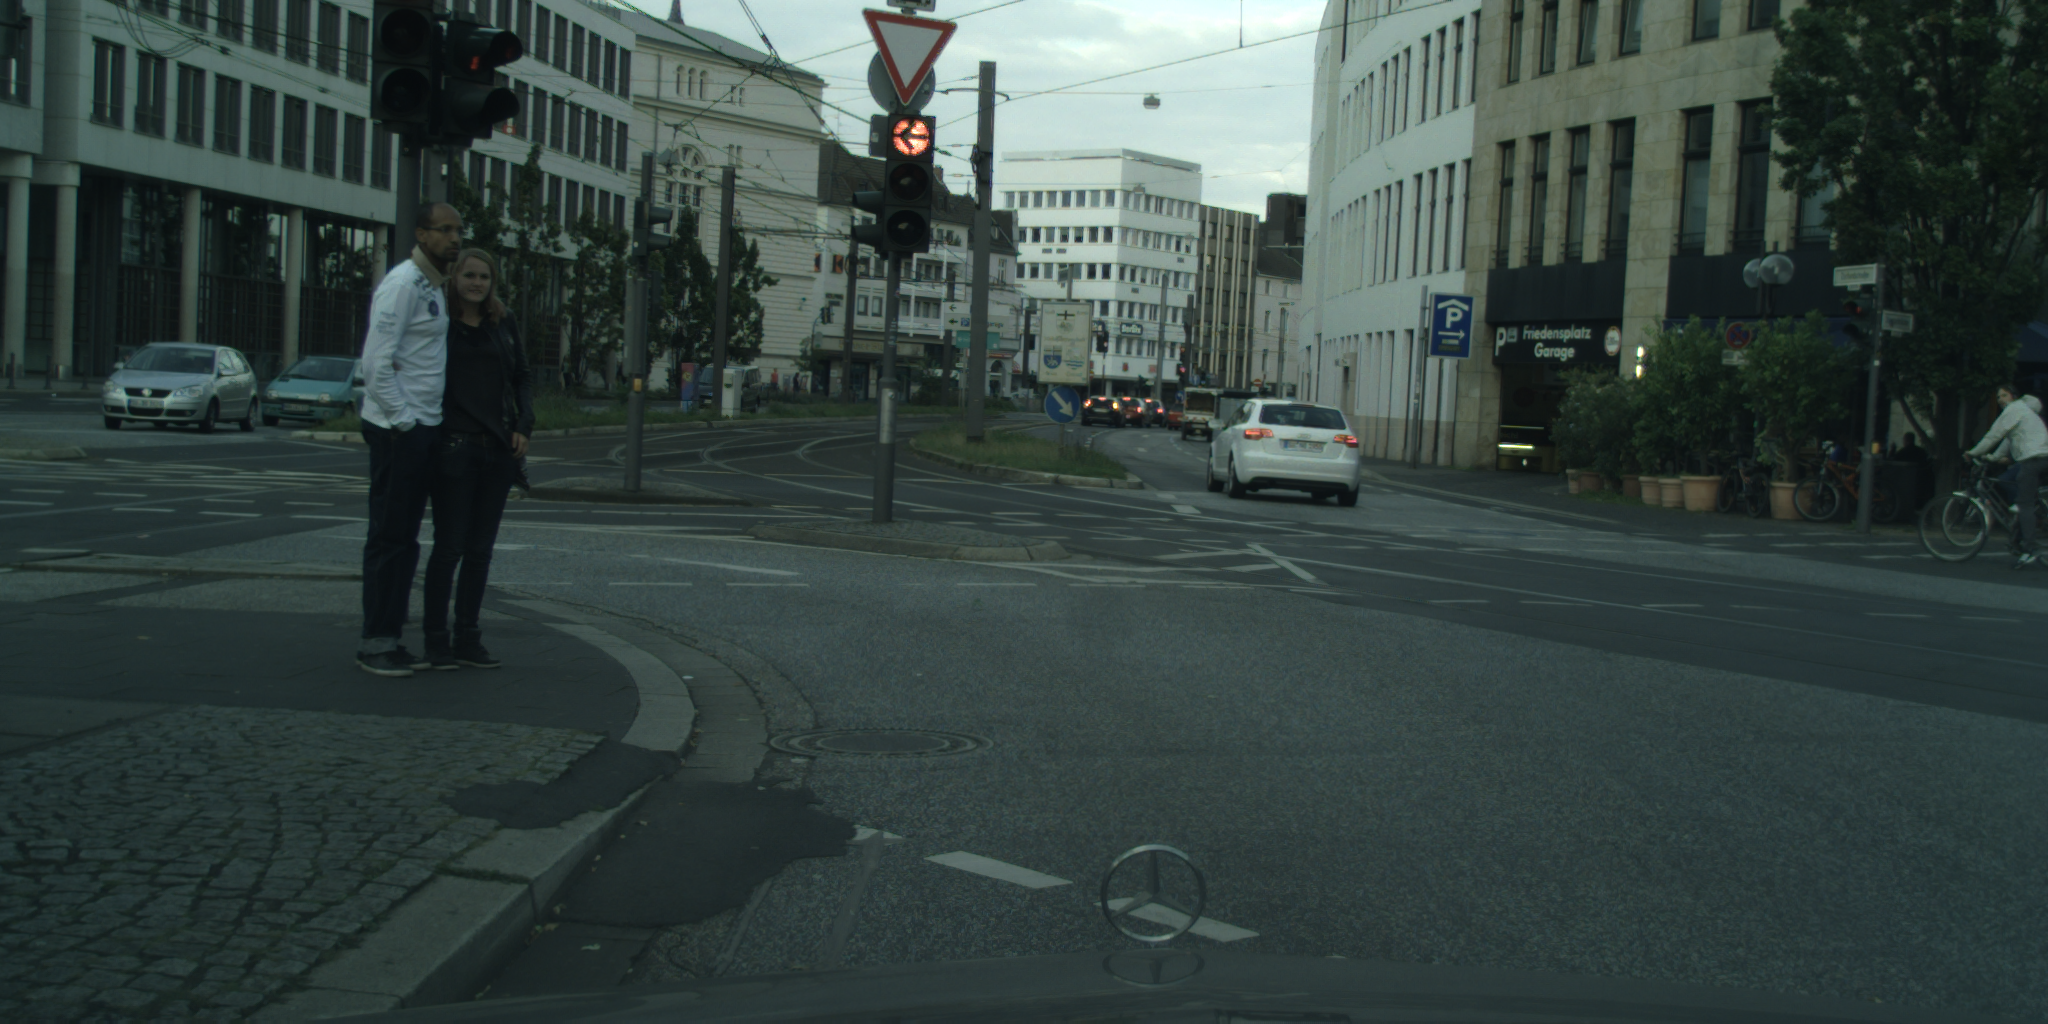
\includegraphics[width=1\linewidth]{figures/bonn_000035_000019_leftImg8bit_original}
    \caption{Picture Bonn35 }
    \label{fig:bonn35}
\end{figure}

On which the models prediction can be observed in the image: Figure\ref{fig:detbonn35}.
\begin{figure}[h]
    \centering
    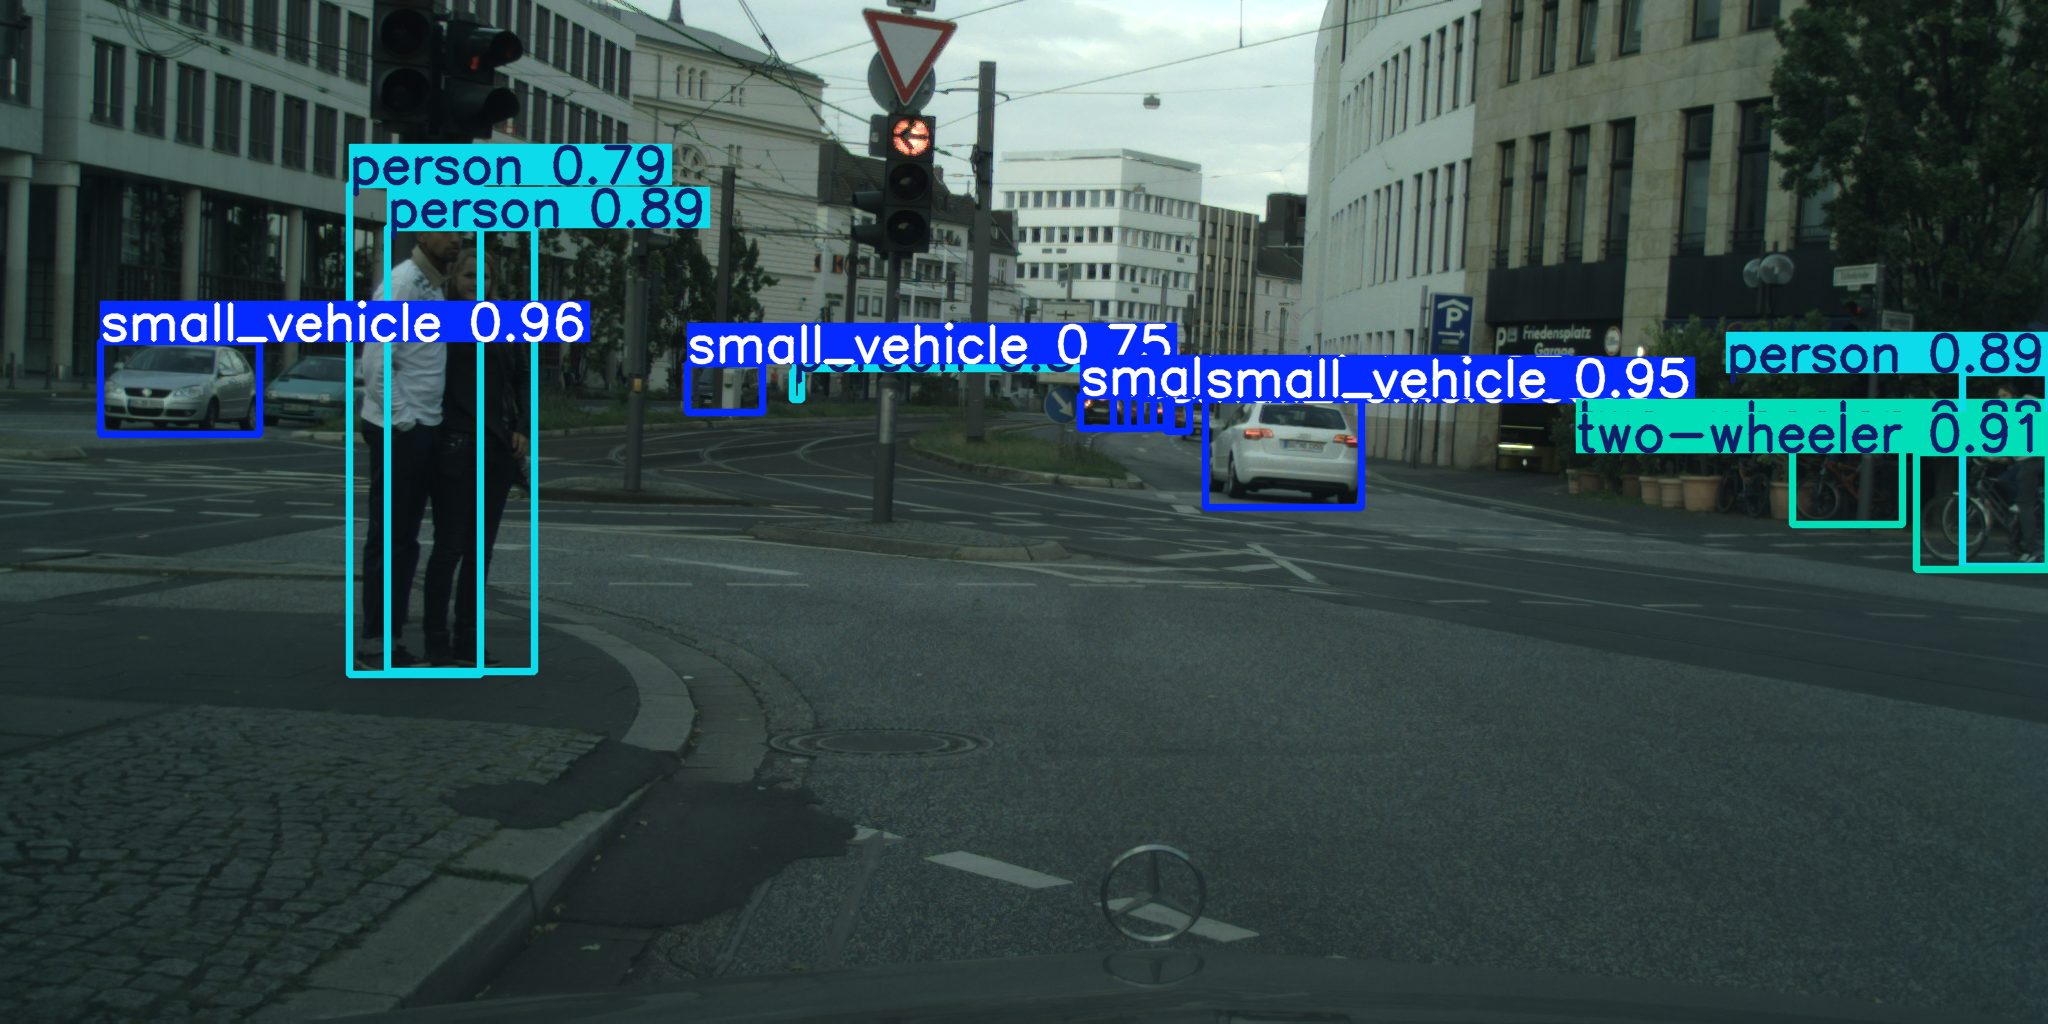
\includegraphics[width=1\linewidth]{figures/bonn_000035_000019_leftImg8bit}
    \caption{Model's detection to the picture Bonn35 }
    \label{fig:detbonn35}
\end{figure}

In the followings I will describe all the image interpretations given by the different interpretation methods. And try and interpret the model's workings based on those outputs.

\newpage

\subsubsection{Evaluation of the EigenCAM method}\label{subsubsec:evaluation-of-the-eigencam-method}

In this figure constellation of Figure\ref{fig:Bonn_000035_000019} different layers are presented.
These layers are

\begin{table}[h]
    \centering
    \begin{tabular}{|c|c|p{10cm}|}
        \hline
        \textbf{Name} & \textbf{Place} & \textbf{Description} \\
         \hline
         -2 C2f  & Feature Pyramid & A composite layer with Cross-Stage Partial Network (CSP) structure, designed to increase gradient flow and reduce memory usage by splitting the feature maps and merging them at the end. \\
         \hline
         -3 Concat & Feature Aggregation & Concatenates feature maps from different scales or layers to merge information, enabling multi-scale predictions. \\
         \hline
         -4 Conv & Convolutional Layer & A standard 2D convolution layer that extracts features from the input by applying filters to generate feature maps. \\
         \hline
         -5 C2f  & Backbone Stage & Similar to the C2f layer at -2, it is responsible for feature extraction with a CSP-like structure to improve computational efficiency and gradient flow. \\
         \hline
    \end{tabular}
    \caption{Yolov8 architecture layers and their descriptions.}
    \label{tab:yolov8_layers}
\end{table}

\begin{figure}[h]
    \centering


    \begin{subfigure}[b]{0.47\textwidth}
        \centering
        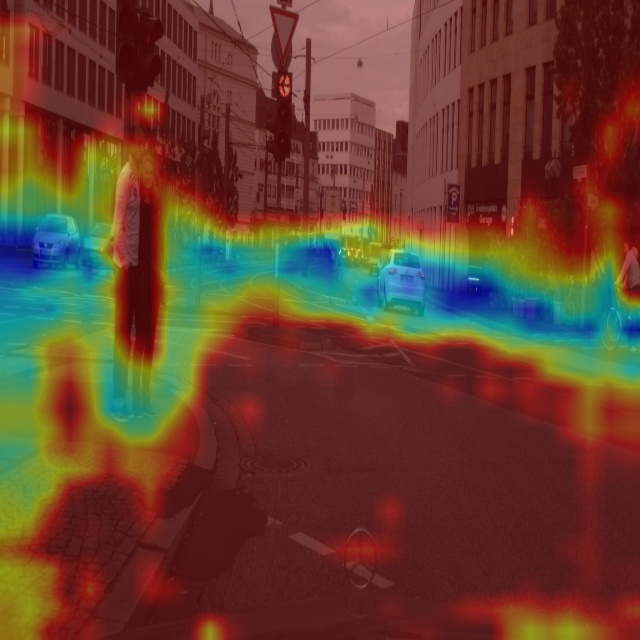
\includegraphics[width=\textwidth]{figures/bonn_000035_000019_leftImg8bit.pnglayer-2/bonn_000035_000019_leftImg8bit.png_object(0)_heatmap}
        \caption{Layer -2}
        \label{fig:a-2}
    \end{subfigure}
    \hfill
    \begin{subfigure}[b]{0.47\textwidth}
        \centering
        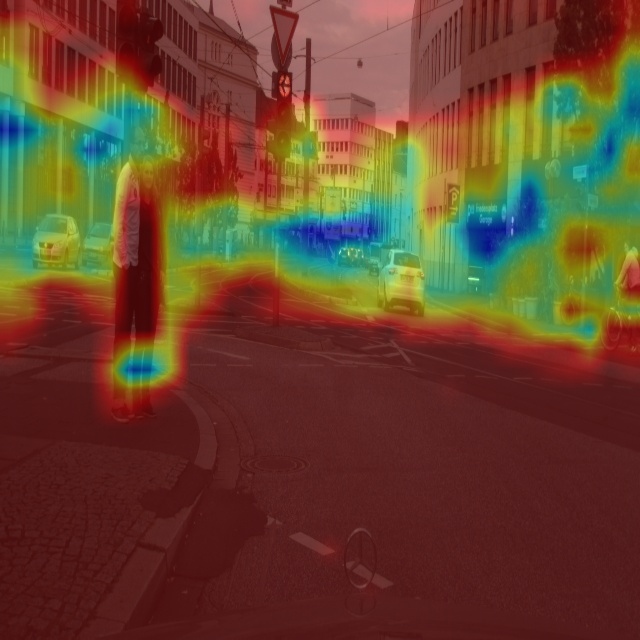
\includegraphics[width=\textwidth]{figures/bonn_000035_000019_leftImg8bit.pnglayer-3/bonn_000035_000019_leftImg8bit.png_object(0)_heatmap}
        \caption{Layer -3}
        \label{fig:-3}
    \end{subfigure}\\
    \hfill
    \begin{subfigure}[b]{0.49\textwidth}
        \centering
        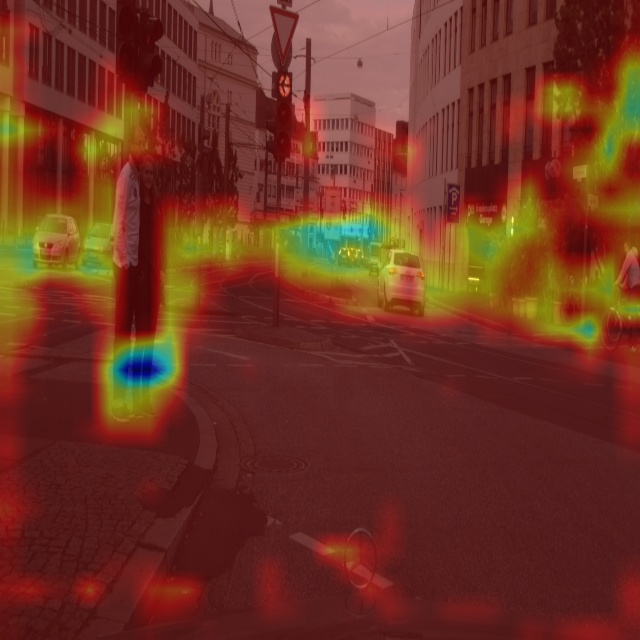
\includegraphics[width=\textwidth]{figures/bonn_000035_000019_leftImg8bit.pnglayer-4/bonn_000035_000019_leftImg8bit.png_object(0)_heatmap}
        \caption{Layer -4}
        \label{fig:-4}
    \end{subfigure}
    \hfill
    \begin{subfigure}[b]{0.49\textwidth}
        \centering
        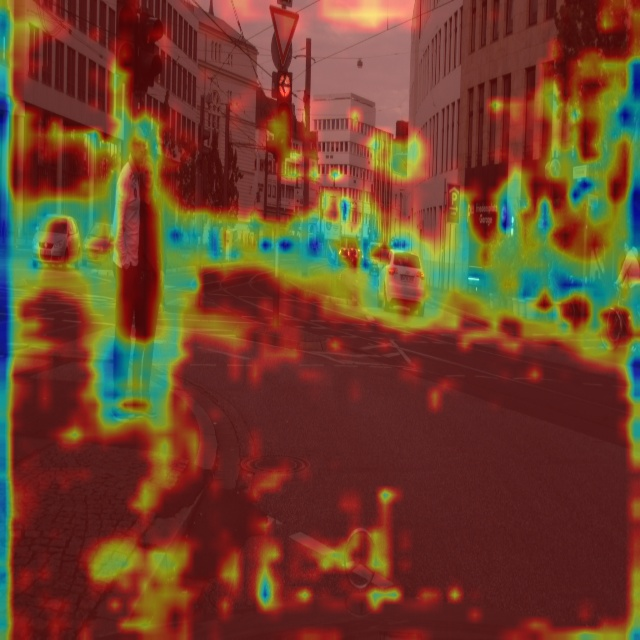
\includegraphics[width=\textwidth]{figures/bonn_000035_000019_leftImg8bit.pnglayer-5/bonn_000035_000019_leftImg8bit.png_object(0)_heatmap}
        \caption{Layer -5}
        \label{fig:-5}
    \end{subfigure}
    \hfill

    \caption{Activation maps for the Layer -2, -3, -4, -5 of Bonn35}
    \label{fig:Bonn_000035_000019}
\end{figure}

The images can be read and interpreted by identifying the layer responsible for each process and observing the colours on the provided activation maps.
The colour red represents the lowest value of activation, while blue represents the highest.
The range of layers observed spanned from the second to last layer to the fifth to last layer,
allowing for the finest resolution of the head to be observed.
This enabled the creation of a visualisation of the areas that were particularly useful in the detection process.

It is evident that the highest activation values were present in the regions where traffic-related objects were identified.
Pedestrians were observed to have their outlines and legs presented with higher activation values.
Additionally, it was noted that the rough edges from the more inner layers in the network exhibited a process of smoothening layer to layer.

\subsubsection{Evaluation of the LIME method}\label{subsubsec:evaluation-of-the-lime-method}
In the figure constellation of Figure\ref{fig:LIME1} and~\ref{fig:LIME2} different types of LIME functions are presented.
These are LIME\_SUM and LIME\_MULTI\@.
LIME\_MULTI aggregates the contributions of each feature across multiple instances by summing the importance scores.
This approach provides a simplified, overall view of how certain features influence the decisions of the model on average,
making it easier to identify the most significant features contributing to the predictions in a broad sense.
LIME\_SUM, on the other hand, focuses on explaining predictions at a finer level.
It applies LIME to multiple instances individually and then analyses the distribution of feature importance across these instances.
This method captures more granular information, allowing for a more detailed understanding of feature interactions and their varying contributions across different samples.

\begin{figure}[h]
    \centering
    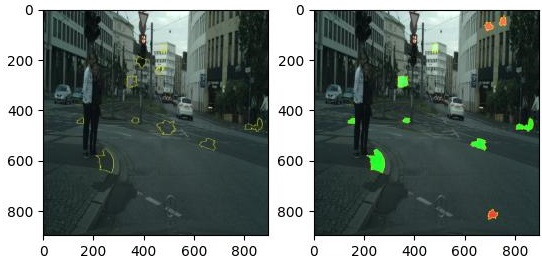
\includegraphics[width=\textwidth]{figures/best-box_bonn_000035_000019_leftImg8bit}
    \caption{LIME\_SUM}
    \label{fig:LIME1}
\end{figure}
\hfill
\begin{figure}[h]
    \centering
    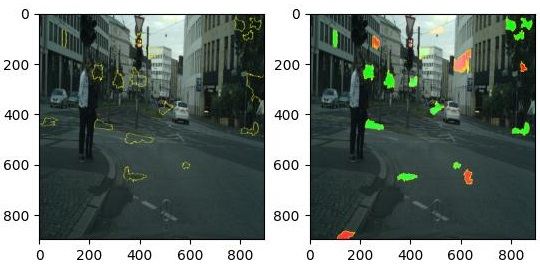
\includegraphics[width=\textwidth]{figures/best-box_bonn_000035_000019_leftImg8bit_MULTI}
    \caption{LIME\_MULTI}
    \label{fig:LIME2}
\end{figure}

The method in question lacks the required granularity and is unable to keep up with more complex neural networks.
Consequently, the resulting output is of questionable reliability, exhibiting inconsistencies such as the appearance of greens adjacent to detected objects, multiple artifacts, and a lack of discernible pattern or rationale in the red markings.
This may be attributed to the method's inherent limitations in providing accurate explanations for intricate problems.

\subsubsection{Evaluation of the SHAP method}\label{subsubsec:evaluation-of-the-shap-method}
In the figure\ref{fig:SHAP_result} SHAP is run to the image, and the shap values are clearly visible on the pictures, each picture represents the run on one instance of detected object.

\begin{figure}[h]
    \centering
    \begin{subfigure}[b]{\textwidth}
        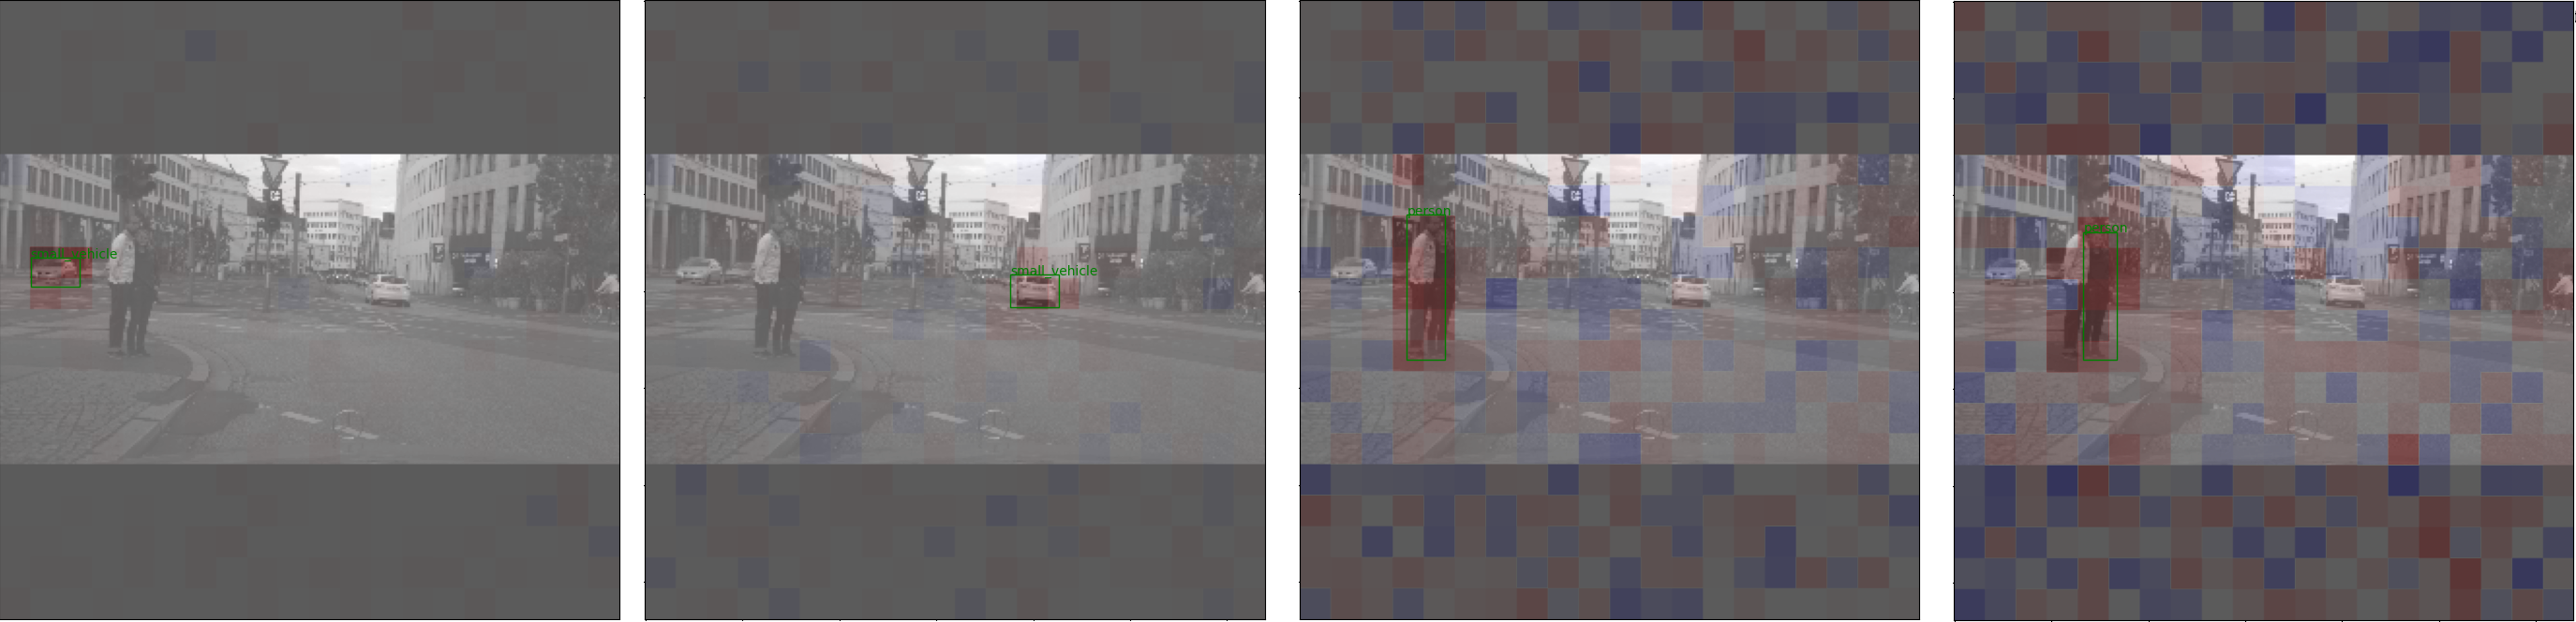
\includegraphics[width=\textwidth]{figures/output1}
        \caption{Shapley values of foreground objects}\label{fig:SHAP_results11}
    \end{subfigure}
    \hfill
    \begin{subfigure}[b]{\textwidth}
        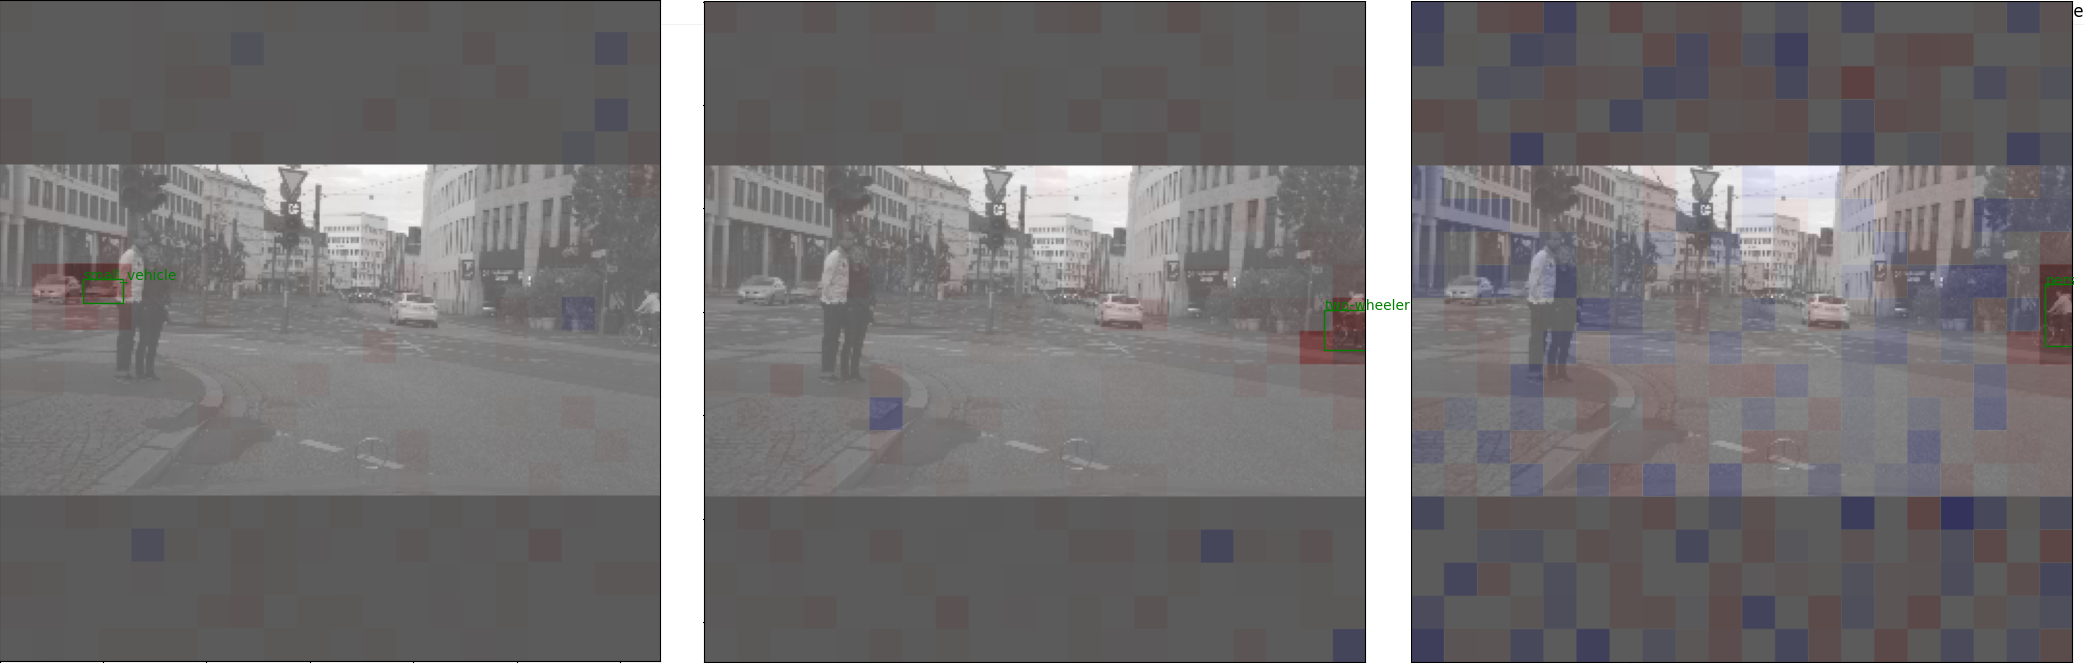
\includegraphics[width=\textwidth]{figures/output1,2}
        \caption{Shapley values of background objects}\label{fig:SHAP_results12}
    \end{subfigure}
    \hfill
    \caption{SHAP results for different instances in Bonn35}
    \label{fig:SHAP_result}
\end{figure}


Red representing higher positive SHAP values, while blue represents negative SHAP values.
Considering the most of the pictures, especially where overrepresented, highly visible objects can be seen, the interpretation is clean and readable.


The SHAP results in both rows (on Figure\ref{fig:SHAP_result} a and b) provide the following insights into the behaviour of the model in this traffic scenario:

\begin{itemize}
\item The uniform highlighting of pedestrians and vehicles across all images indicates that the model is effectively identifying and focusing on the critical elements within the traffic scene. This is an encouraging indication of the interpretability of the model and reliability in detecting important objects.
\item The absence of emphasis on or attention to the muted or cooler blocks on buildings and other background areas indicates that the model does not rely on these features for its predictions. This is an anticipated and favourable outcome in the context of traffic-related tasks.
\item Additionally, an anomaly is is evident on the more \("\)noisy\("\) images, which may be a limitation of this methodology.
\end{itemize}




\subsection{Addressing the Anomaly regarding the noise of SHAP and the probability of the models detection}\label{subsec:Addressing the Anomaly regarding SHAP and the probability of detection}
% Detekció bizonyossága vs interpretáció zajosság

As previously stated in the previous subsection~\ref{subsec:evaluation-of-interpretation-methods},
the SHAP values for objects with lower detection probability are characterised by a high degree of noise,
rendering them unable to provide a clear and coherent explanation for the predictions of the model.
This anomaly can be attributed to the low probability of detection for this instance pedestrian class, which results in unreliable,
often contradicting information for the SHAP algorithm to interpret.
This phenomenon is common in object detection models, where the detection accuracy for small objects is lower than that for larger or more clearly visible objects.
Furthermore, as previously discussed in section~\ref{par:adversarial-based-interpretation} that the detection threshold of this model and the probability of detection can
have a significant impact on the actual decision-making process of the model.
The combination of perturbation-based interpretation methods may result in unreliable and noisy results, as the perturbed image segments may be misclassified by the model.

Furthermore, an additional cause of this noise can be identified, which is more comprehensible when considering the proportions of the various classes of traffic objects present in the dataset.
As illustrated in Figure~\ref{fig:Label_distribution} the dataset exhibits a significant class imbalance, with certain classes, such as vehicles, being overrepresented in comparison to others, such as pedestrians.
This imbalance may result in the generation of noise in the interpretations, as the model may exhibit a tendency to favour the more frequent classes due to the larger volume of data from which it has learned.
Consequently, the limited number of examples for less frequent classes, such as pedestrians, may not provide the model with sufficient information to effectively capture their distinctive and often subtle features.

\begin{figure}[ht]
    \centering
    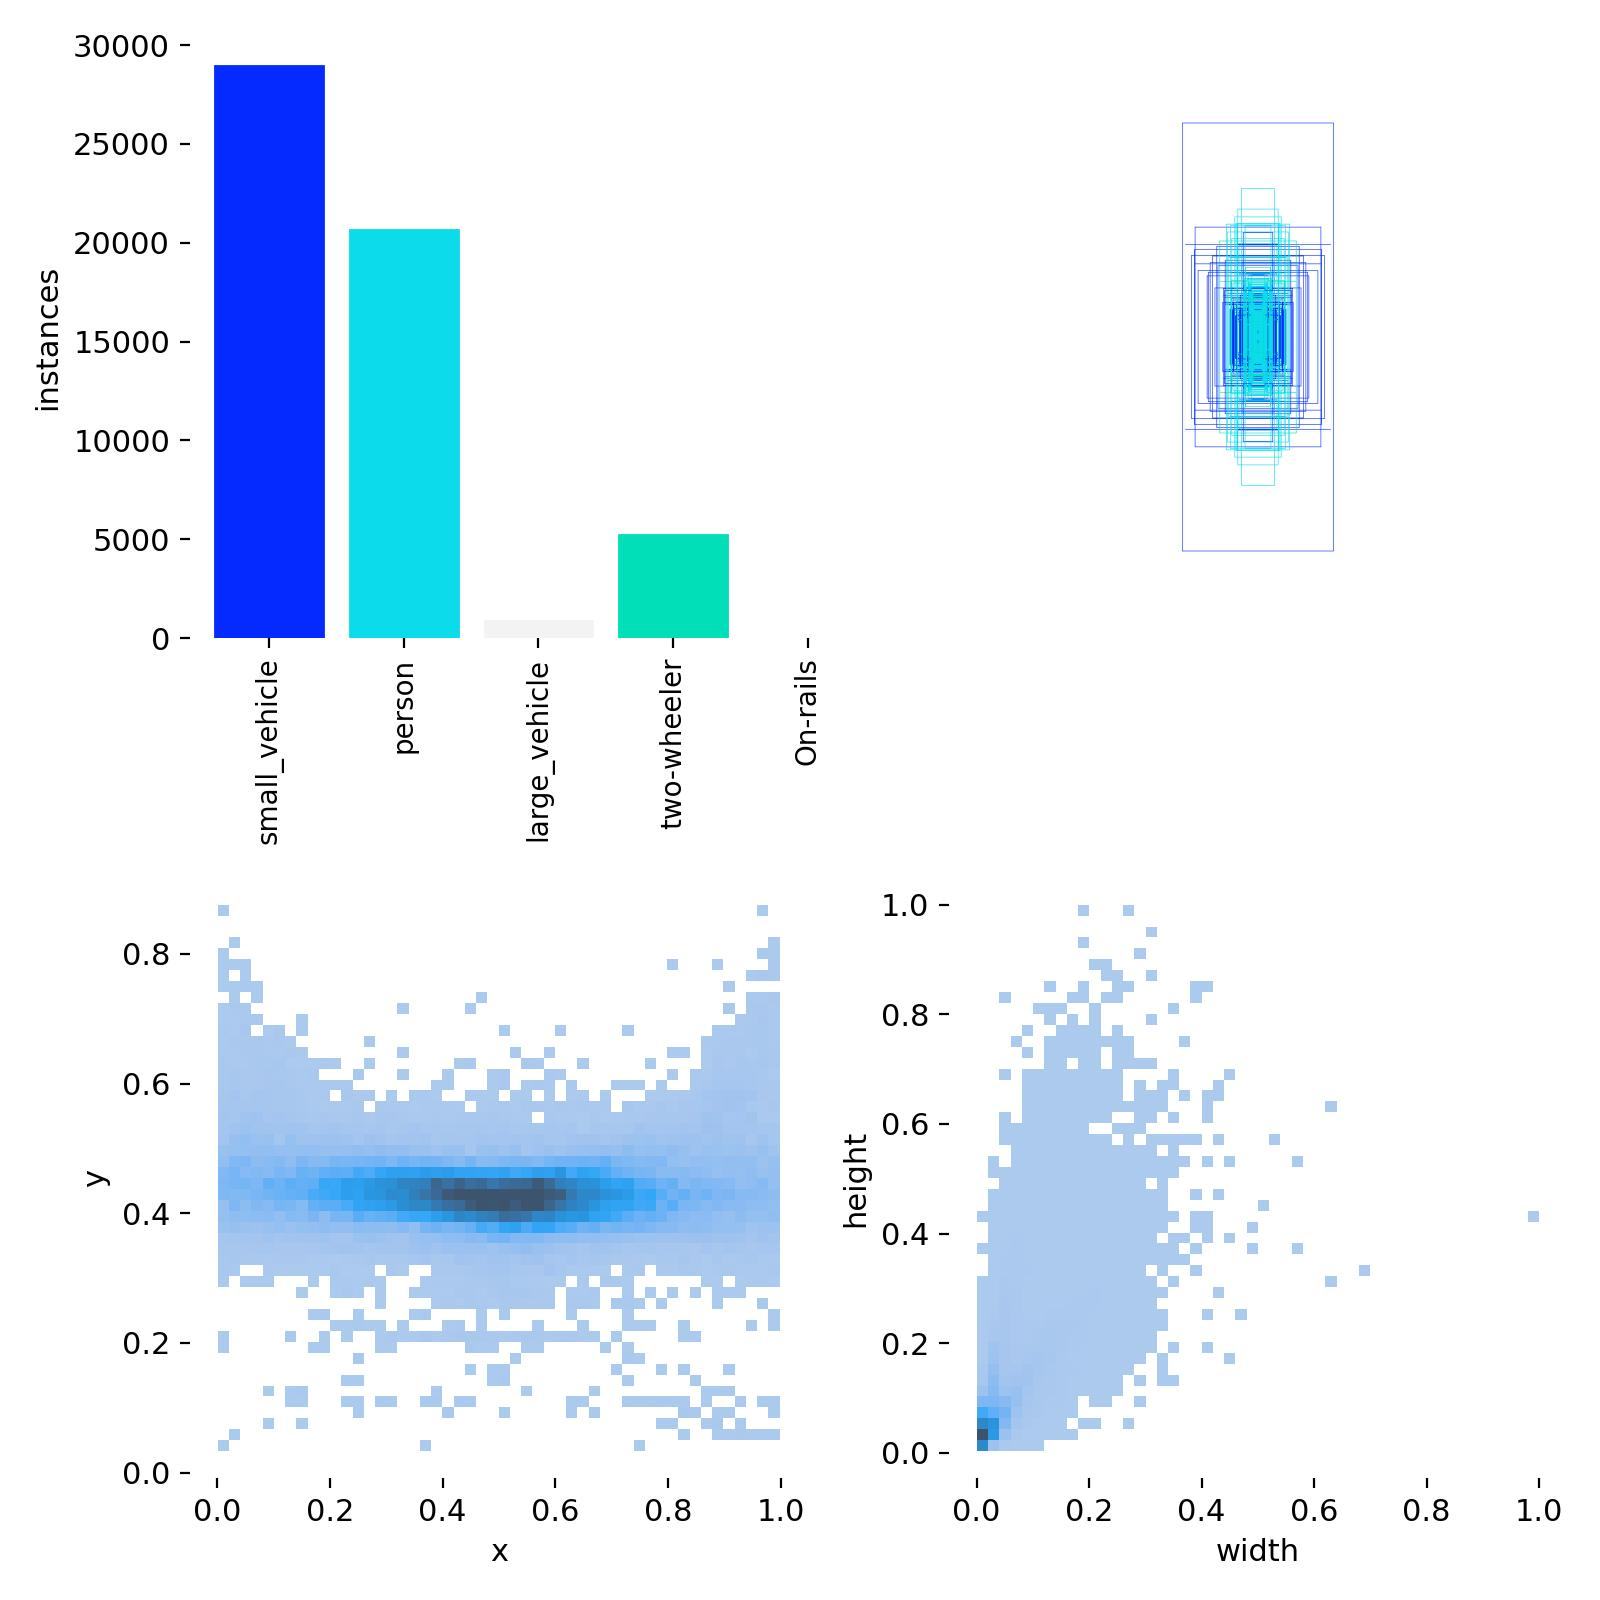
\includegraphics[width=0.8\linewidth]{figures/labels-30}
    \caption{Label distribution}
    \label{fig:Label_distribution}
\end{figure}

This deficiency in the training data can give rise to a number of issues.
For example, the model may encounter difficulties in generalising effectively when it encounters pedestrian objects in real-world scenarios, due to insufficient exposure to their diverse appearances and contexts during training.
Consequently, the model may miss-classify or fail to identify pedestrians, which can introduce additional noise in its output, manifesting as false negatives or incorrect predictions.(This is represented on Figure~\ref{fig:Confusionmatrix})
Furthermore, the distinctive characteristics that differentiate pedestrian objects, such as specific shapes, movements, or interactions with the environment, may be under-represented in the model's learned representations.
To mitigate this noise and enhance detection accuracy, it is essential to balance the dataset or augment it with more diverse examples of the minority class, thereby enhancing the model's ability to learn these crucial features effectively.

\begin{figure}
    \centering
    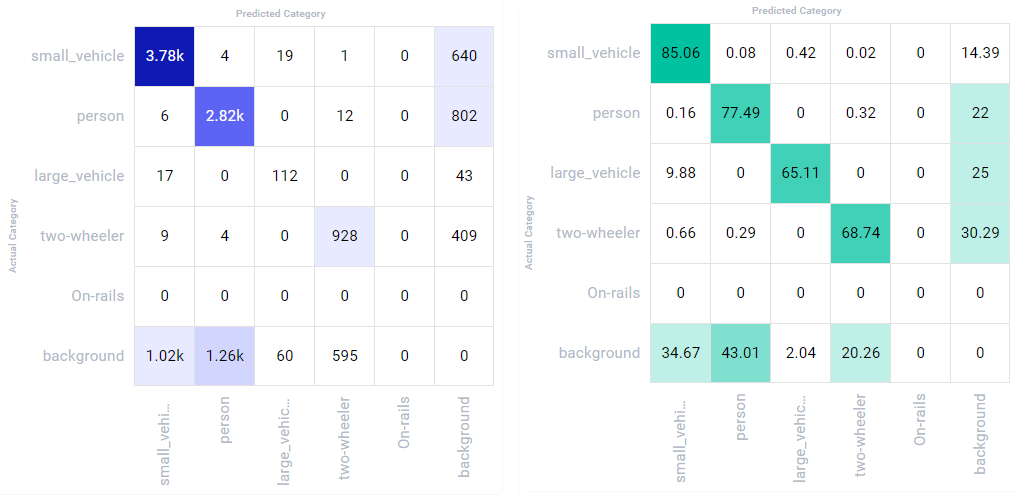
\includegraphics[width=1\linewidth]{figures/confusion_matrix2}
    \caption{Confusion matrix showing the us the detailed classification results of an algorithm on a test set by analysing its rows, columns, or entries}
    \label{fig:Confusionmatrix}
\end{figure}
%% külön cm-ről

The provided image presents two confusion matrices, one with absolute values and the other with percentages, which elucidate pivotal aspects of the model's performance.

To address this issue, an increase in the detection threshold of the model for the class of noisy object  may be beneficial in improving the detection probability of already detected objects.
This could be achieved by ignoring detections with a lower probability, thus enhancing the reliability and decreasing the noise
of SHAP interpretations.
This adjustment can help reduce the noise but may also result in the exclusion of some objects from the interpretation process.
Making the interpretation process more incompletely, but more reliable and less noisy.

\subsubsection{Explanations to the Confusion Matrix}
The confusion matrices provide a detailed assessment of the model's classification performance for categories: \textit{small\_vehicle}, \textit{person} and \textit{large\_vehicle}.

The absolute score matrix (left) shows high accuracy for \textit{small\_vehicle} (3,780 correct) and \textit{person} (2,820 correct), but also reveals misclassifications, such as 640 \textit{small\_vehicle} instances identified as \textit{background}. Similarly, the class \textit{two-wheeler} has 928 correct classifications, but some confusion with \textit{background}.

The percentage matrix (right) normalises these results and shows high accuracy for \textit{small\_vehicle} (85.06\%) and \textit{person} (77.49\%), while \textit{two wheeler} accuracy drops to 68.74\% due to misclassification (30.29\% as \textit{background}). The \textit{background} category also shows considerable confusion with other classes.

These matrices highlight strengths and weaknesses, guiding improvements in preprocessing, model design, and training while enhancing result interpretability—a core focus of this thesis.
\newpage


